\documentclass[12pt,a4paper,oneside]{article}

% Packages
\usepackage{listings}
\usepackage{color}
\usepackage{graphicx}
\usepackage[a4paper,left=2cm,right=2cm,top=2cm,bottom=2.5cm]{geometry}

% Set up listings package for code
\lstdefinestyle{ElliottCListingStyle}{
  language=C,
  numbers=left,
  stepnumber=1,
  numbersep=10pt,
  tabsize=4,
  showspaces=false,
  showstringspaces=true
}

% Title Set Up
\title{Practical Write Up}
\author{Elliott Rarden}
\date{\today}

\begin{document}

% Title
\maketitle

\section{Practical 1 - Pipes and Forks}
\subsection{Question 1}
In the OSX implementation of fork(), processes do not call clone, so I cannot answer the expert question for this question.  Instead, I will discuss why Mac OS does this. fork()'s implementation on OSX is tied directly to the system's underlying process manager, Grand Central Dispatch (GCD).  Apple's engineers chose to use the fork() system call over clone() to work with GCD.  
\subsubsection{Strace output from Beej's code}
\begin{verbatim}
$ sudo dtruss -acf -t process -t pipe ./beej

  PID/THRD       RELATIVE   ELAPSD   CPU   SYSCALL(args)             = return
50591/0x8b0399:      6394        8     5   pipe(0x2, 0xC59F, 0x11)   = 3
50592/0x8b03a8:       109        0     0   fork()                    = 0

CALL                                        COUNT
fork                                            1 // GCD at work
ioctl                                           1
munmap                                          1
pipe                                            1 // Pipe is created
proc_info                                       1
shared_region_check_np                          1
bsdthread_register                              2
dup                                             2 // Streams are copied
execve                                          2
fcntl                                           2
getpid                                          2
issetugid                                       2
pread                                           2
sysctl                                          2
csops                                           3
open                                            3 // FILE* is fun
thread_selfid                                   3
mmap                                            4 // Streams are set in memory
close                                           7
mprotect                                        8
\end{verbatim}
\newpage

\subsection{Question 2}
Any process can talk to any other if they set up the correct pipes.  This is incredibly common in UNIX scripting.  Pipes can even go to files (they are all FILE* in the end anyway)
\begin{verbatim}
$ ls -al > currentDirectoryListing.txt
\end{verbatim}

\subsubsection{My code for fork/pipe}
\begin{lstlisting}[basicstyle=\scriptsize, style=ElliottCListingStyle]
#include <stdio.h>
#include <stdlib.h>
#include <unistd.h>

int main(void)
{
	// index 0 = read
	// index 1 = write
	int pipe1[2];
	int pipe2[2];
	pipe(pipe1);
	pipe(pipe2);

	if (!fork()) // New process created here, it starts after the else
	{ 	// Process 0

		// There is no input from pipe1, close it's input
		close(pipe1[0]);

		// Set stdout to pipe1
		close(1);
		dup(pipe1[1]);

		// Make call
		execlp("cat", "cat", "/etc/passwd", NULL);
	}
	else // the process created here spawns into two processes
	{
		if (!fork()) // Same as above, new process starts after the else
		{	// Process 1

			// Set standard input from pipe1
			close(0);
			dup(pipe1[0]);

			// set stdout to pipe2
			close(1);
			close(pipe1[1]);
			dup(pipe2[1]);

			// Make call
			execlp("cut", "cut", "-f1", "-d:", NULL);
		}
		else
		{	// Process 2

			// Set standard input from pipe2
			close(0);
			close(pipe1[0]);
			dup(pipe2[0]);

			// There is no output to pipe1 or pipe2
			close(pipe1[1]);
			close(pipe2[1]);

			// Make call
			execlp("sort", "sort", NULL);
		}
	}
	// Done
	return 0;
}
\end{lstlisting}

\newpage

\subsubsection{Strace output from my code}
\begin{verbatim}
  PID/THRD       RELATIVE   ELAPSD   CPU   SYSCALL(args)             = return
50708/0x8b2613:      5732       11     6   pipe(0x2, 0xC614, 0x11)   = 3
50708/0x8b2613:      5736        5     3   pipe(0x2, 0xC614, 0x11)   = 5
50709/0x8b2623:        74        0     0   fork()                    = 0
50710/0x8b2624:        72        0:    0   fork()                    = 0

CALL                                        COUNT
fstat64                                         1
ioctl                                           1
munmap                                          1
proc_info                                       1
shared_region_check_np                          1
fcntl                                           2
fork                                            2 // Created 2 children
getpid                                          2
issetugid                                       2
pipe                                            2 // Creating pipes
pread                                           2
sysctl                                          2
bsdthread_register                              3
    // Arch BSD's Motto - "only after a few drinks"
csops                                           3
execve                                          3
open                                            3
dup                                             4 // Opening FILE*
mmap                                            4
thread_selfid                                   4
mprotect                                        8
    // GCD is really cool, it protects your children when you don't
close                                          12 // You open 4, you close 8
stat64                                         45
\end{verbatim}

\newpage

\section{Practical 2 - Concurrency}
\subsection{Question 1 - Concurrent processes}
Multiple processes can have 100\% processor usage if your machine has more than one physical core.  Since the process queue can distribute its workload to multiple processors, they can each have 100\% of a given core.  You can use this knowledge to determine how many cores a processor has.  Start by setting N equal to 2.  If both processes reach ~100\%, then increase N to 4.  Again, if both processes reach ~100\%, increase N to 8.  Repeate until the processes have a value less than 100\%.  The largest number where the processors do not reach ~100\% is the number of cores.
\subsubsection{Table of processor usage for Question 1}
\begin{center}
\begin{tabular}{|l|l|}
\hline
N (Number of Processes) & Approx Processor Usage (\% per process) \\ \hline
2                       & 100\%                                   \\ \hline
4                       & 100\%                                   \\ \hline
8                       & 50\%                                    \\ \hline
16                      & 25\%                                    \\ \hline
\end{tabular}
\end{center}

\newpage

\subsection{Question 2}
\subsubsection{Code for Question 2}
\begin{lstlisting}[basicstyle=\scriptsize, style=ElliottCListingStyle]
#include <unistd.h>
#include <pthread.h>
#include <stdio.h>
#include <stdlib.h>
#include <math.h>

#define NUM_THREADS 2 /* define the total number of Threads we want */

/* Set global variable */
float total=0;

/* compute function just does something. */
void *compute()
{
	int i;
	float oldtotal=0, result=0;

	/* for a large number of times just square root and square
	the arbitrary number 1000 */
	for(i=2000000000;i!=0;i--)
	{
		result=sqrt(1000.0)*sqrt(1000.0);
	}

	/* Print the result ? should be no surprise */
	printf("Result is %f\n",result);

	/* We want to keep a running total in the global variable total */
	oldtotal = total;
	total = oldtotal + result;

	/* Print running total so far. */
	printf("Total is %f\n",total);

	pthread_exit(NULL);
}

int main()
{
	pthread_t threads[NUM_THREADS];
	int i;
	int retcodes[NUM_THREADS];
	float result=0;

	printf("\n"); /* bit of whitespace */

	/* Create the proper number of threads */
	for(i=0; i<NUM_THREADS; i++)
	{
		/* give a message about which thread we're creating */
		printf("Creating Thread #%d\n", i);

		/* Create the thread */
		retcodes[i] = pthread_create(&threads[i], NULL, compute, NULL);

		if (retcodes[i]) // If pthread_create gave us a value that isn't 0
		{
			printf("ERROR; return code from pthread_create() is %d\n", retcodes[i]);
			exit(-1); // Shit hit the fan
		}
	}

	pthread_exit(NULL);

	/* nothing else to do so end main function (and program) */
	return 0;
}
\end{lstlisting}
\newpage

\subsection{Question 3}
The difference in behaviour is that the threaded program keeps a running total between all of the threads, whereas the one with processes does not.  This is because fork() creates an exact copy of the entire program, including the data section which includes global variables.  The threaded version does not copy these, and instead, each thread uses the primary programs memory pool.

\subsection{Question 4}
The critical section is where the variable is updated.
\subsubsection{Code for Question 4}
From above, replace line 30 with
\begin{lstlisting}[basicstyle=\small, style=ElliottCListingStyle]
	/* Critical Section - add POSIX semaphore */
	#if USE_SEMAPHORES != 0
		sem_wait(&mutex);
		total = oldtotal + result;
		sem_post(&mutex);
	#else
		total = oldtotal + result;
	#endif
\end{lstlisting}

Add the following to \texttt{main()} before the \texttt{for} loop

\begin{lstlisting}[basicstyle=\small, style=ElliottCListingStyle]
	#if USE_SEMAPHORES != 0
		// Initialise the semaphore
		sem_init(&mutex, 0, 1);
	#endif
\end{lstlisting}

And add the following after the \texttt{pthread\_exit(NULL);} statement

\begin{lstlisting}[basicstyle=\small, style=ElliottCListingStyle]
	#if USE_SEMAPHORES != 0
		/* Once all threads are merged, we can destroy the semaphore */
		sem_destroy(&mutex);
	#endif
\end{lstlisting}

You will also need to declare the following globally, near the top of the file

\begin{lstlisting}[basicstyle=\small, style=ElliottCListingStyle]
	// Partial compilation
	#define USE_SEMAPHORES 1

	#if USE_SEMAPHORES != 0
		// Initialise the semaphore
		sem_t mutex;
	#endif
\end{lstlisting}
You can enable or disable the semaphore by setting \texttt{USE\_SEMAPHORES} before compilation to either 1 (enable) or 0 (disable).  
\newpage

\section{Practical 3 - Interprocess Communication}

\subsection{Question 1}
\subsubsection{kirk2.c}

\begin{lstlisting}[basicstyle=\scriptsize, style=ElliottCListingStyle]
/*
** kirk2.c -- writes to a message queue
*/

#include <stdio.h>
#include <stdlib.h>
#include <errno.h>
#include <string.h>
#include <sys/types.h>
#include <sys/ipc.h>
#include <sys/msg.h>

// Message Types
#define URGENT (1)
#define NORMAL (2)

struct my_msgbuf {
	long mtype;
	char mtext[200];
};

int main(void)
{
	struct my_msgbuf buf;
	int msqid;
	key_t key;

	if ((key = ftok("kirk.c", 'B')) == -1) {
		perror("ftok");
		exit(1);
	}

	if ((msqid = msgget(key, 0644 | IPC_CREAT)) == -1) {
		perror("msgget");
		exit(1);
	}
	
	printf("Enter lines of text, ^D to quit:\n");

	while(fgets(buf.mtext, sizeof buf.mtext, stdin) != NULL) {
		int len = strlen(buf.mtext);

		/* ditch newline at end, if it exists */
		if (buf.mtext[len-1] == '\n')
			buf.mtext[len-1] = '\0';

		/* Check and set message type */
		if (len > 6 && (strncmp("URGENT", buf.mtext, 6) == 0) )
			buf.mtype = URGENT;
		else
			buf.mtype = NORMAL;

		if (msgsnd(msqid, &buf, len+1, 0) == -1) /* +1 for '\0' */
			perror("msgsnd");
	}

	if (msgctl(msqid, IPC_RMID, NULL) == -1) {
		perror("msgctl");
		exit(1);
	}

	return 0;
}
\end{lstlisting}
\newpage
\subsubsection{starfleet.c}
\begin{lstlisting}[basicstyle=\scriptsize,style=ElliottCListingStyle]
/*
** starfleet.c -- reads from a message queue
*/

#include <stdio.h>
#include <stdlib.h>
#include <errno.h>
#include <sys/types.h>
#include <sys/ipc.h>
#include <sys/msg.h>

// Message Types
#define URGENT (1)
#define NORMAL (2)

struct my_msgbuf {
	long mtype;
	char mtext[200];
};

int main(void)
{
	struct my_msgbuf buf;
	int msqid;
	key_t key;

	if ((key = ftok("kirk.c", 'B')) == -1) {  /* same key as kirk.c */
		perror("ftok");
		exit(1);
	}

	if ((msqid = msgget(key, 0644)) == -1) { /* connect to the queue */
		perror("msgget");
		exit(1);
	}
	
	printf("starfleet: ready to receive messages, captain.\n");

	for(;;) { /* Spock never quits! */
		if (msgrcv(msqid, &buf, sizeof buf.mtext, URGENT, 0) == -1) {
			perror("msgrcv");
			exit(1);
		}
		printf("starfleet: \"%s\"\n", buf.mtext);
	}

	return 0;
}
\end{lstlisting}

\newpage
\subsection{Question 2}
\subsubsection{kirk3.c}
\begin{lstlisting}[basicstyle=\tiny, style=ElliottCListingStyle]
/*
** kirk3.c -- teleportation?
*/

#include <stdio.h>
#include <stdlib.h>
#include <errno.h>
#include <string.h>
#include <sys/types.h>
#include <sys/ipc.h>
#include <sys/msg.h>
#include <signal.h>

// Message Types
#define URGENT (1)
#define NORMAL (2)

struct my_msgbuf {
	long mtype;
	char mtext[200];
};

volatile sig_atomic_t got_usr1;

void sigusr1_handler(int sig)
{
	got_usr1 = 1;
}

int main(void)
{
	struct sigaction sa;
	got_usr1 = 0;

	sa.sa_handler = sigusr1_handler;
	sa.sa_flags = 0;
	sigemptyset(&sa.sa_mask);
	if (sigaction(SIGUSR1, &sa, NULL) == -1) {
		perror("sigaction");
		exit(1);
	}

	struct my_msgbuf buf;
	int msqid;
	key_t key;

	if ((key = ftok("kirk.c", 'B')) == -1) {
		perror("ftok");
		exit(1);
	}

	if ((msqid = msgget(key, 0644 | IPC_CREAT)) == -1) {
		perror("msgget");
		exit(1);
	}
	
	printf("Enter lines of text, ^D to quit:\n");

	while(fgets(buf.mtext, sizeof buf.mtext, stdin) != NULL && !got_usr1) {
		int len = strlen(buf.mtext);

		/* ditch newline at end, if it exists */
		if (buf.mtext[len-1] == '\n')
			buf.mtext[len-1] = '\0';

		/* Check and set message type */
		if (len > 6 && (strncmp("URGENT", buf.mtext, 6) == 0) )
			buf.mtype = URGENT;
		else
			buf.mtype = NORMAL;

		if (msgsnd(msqid, &buf, len+1, 0) == -1) /* +1 for '\0' */
			perror("msgsnd");
	}

	if (msgctl(msqid, IPC_RMID, NULL) == -1) {
		perror("msgctl");
		exit(1);
	}

	return 0;
}
\end{lstlisting}
\newpage

\begin{figure}[h]
   \centering
   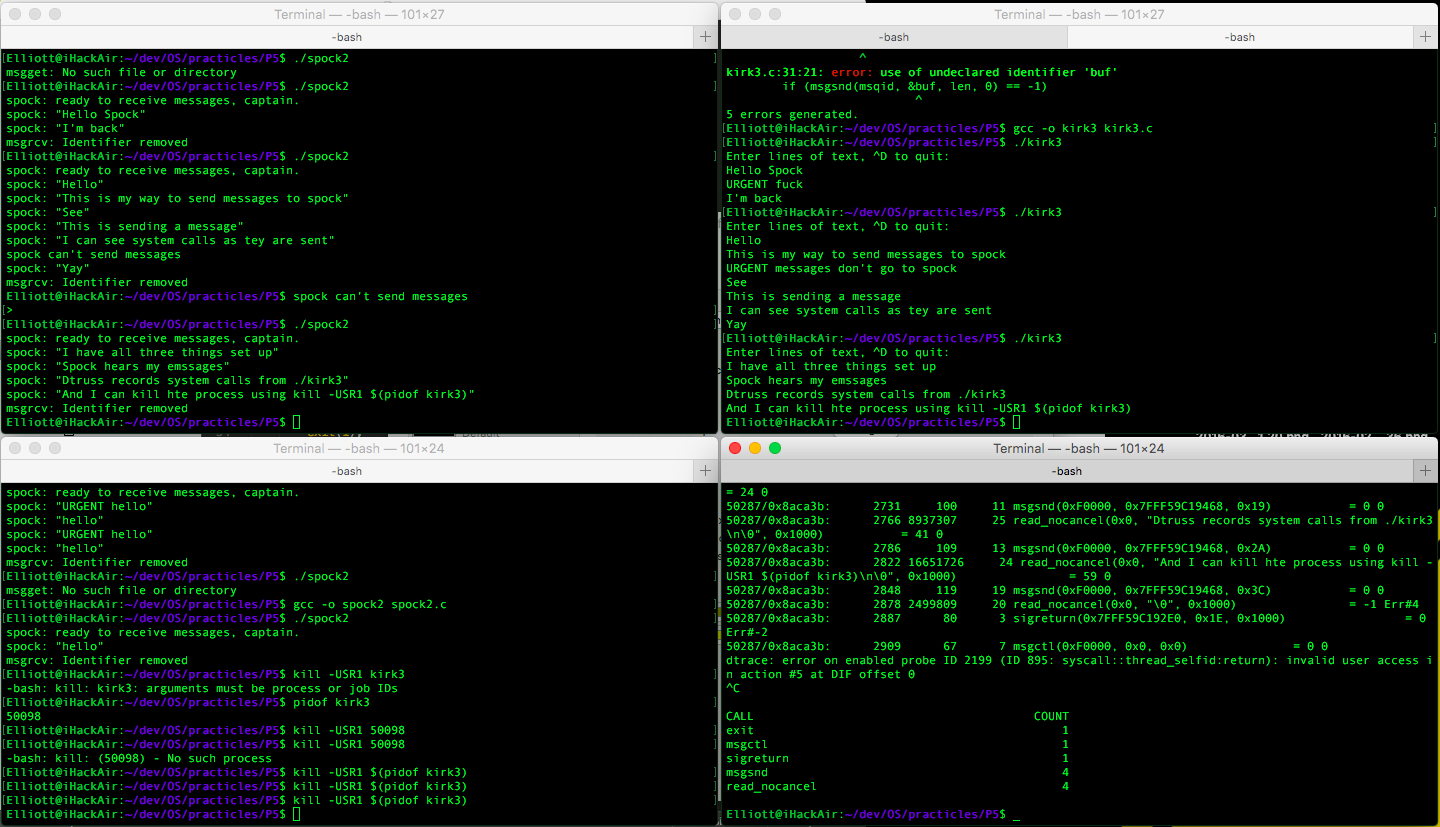
\includegraphics[width=\textwidth]{TerminalWindows.jpg} 
   \caption{Windows clockwise starting in top left: spock.c, kirk3.c, dtruss (OSX strace), BASH (to give kill command).}
   \label{Terminal Windows while running kirk3}
\end{figure}


























\end{document}
